%%%%%%%%%%%%%%%%%%%%%%%%%%%%%%%%%%%%%%%%%
% Beamer Presentation
% LaTeX Template
% Version 1.0 (10/11/12)
%
% This template has been downloaded from:
% http://www.LaTeXTemplates.com
%
% License:
% CC BY-NC-SA 3.0 (http://creativecommons.org/licenses/by-nc-sa/3.0/)
%
%%%%%%%%%%%%%%%%%%%%%%%%%%%%%%%%%%%%%%%%%

%----------------------------------------------------------------------------------------
%	PACKAGES AND THEMES
%----------------------------------------------------------------------------------------

\documentclass[xcolor=dvipsnames]{beamer}

\mode<presentation> {

% The Beamer class comes with a number of default slide themes
% which change the colors and layouts of slides. Below this is a list
% of all the themes, uncomment each in turn to see what they look like.

%\usetheme{default}
%\usetheme{AnnArbor}
%\usetheme{Antibes}
%\usetheme{Bergen}
%\usetheme{Berkeley}
%\usetheme{Berlin}
%\usetheme{Boadilla}
%\usetheme{CambridgeUS}
%\usetheme{Copenhagen}
%\usetheme{Darmstadt}
%\usetheme{Dresden}
%\usetheme{Frankfurt}
%\usetheme{Goettingen}
%\usetheme{Hannover}
%\usetheme{Ilmenau}
%\usetheme{JuanLesPins}
%\usetheme{Luebeck}
\usetheme{Madrid}
%\usetheme{Malmoe}
%\usetheme{Marburg}
%\usetheme{Montpellier}
%\usetheme{PaloAlto}
%\usetheme{Pittsburgh}
%\usetheme{Rochester}
%\usetheme{Singapore}
%\usetheme{Szeged}
%\usetheme{Warsaw}

% As well as themes, the Beamer class has a number of color themes
% for any slide theme. Uncomment each of these in turn to see how it
% changes the colors of your current slide theme.

%\usecolortheme{albatross}
%\usecolortheme{beaver}
%\usecolortheme{beetle}
%\usecolortheme{crane}
%\usecolortheme{dolphin}
%\usecolortheme{dove}
%\usecolortheme{fly}
%\usecolortheme{lily}
%\usecolortheme{orchid}
%\usecolortheme{rose}
%\usecolortheme{seagull}
%\usecolortheme{seahorse}
%\usecolortheme{whale}
%\usecolortheme{wolverine}

%\setbeamertemplate{footline} % To remove the footer line in all slides uncomment this line
%\setbeamertemplate{footline}[page number] % To replace the footer line in all slides with a simple slide count uncomment this line

\setbeamertemplate{navigation symbols}{} % To remove the navigation symbols from the bottom of all slides uncomment this line
}
\setbeamercovered{transparent=50}

\usepackage{graphicx} % Allows including images
\usepackage{booktabs} % Allows the use of \toprule, \midrule and \bottomrule in tables
\usepackage{soul}
\usepackage{xspace}
\usepackage[dvipsnames]{xcolor}
\usepackage{MnSymbol,wasysym}

%%MACROS
\newcommand{\A}{\mathcal A\xspace}
\renewcommand{\L}{\mathcal L\xspace}
\newcommand{\T}{\mathcal T\xspace}
\newcommand{\always}{\mathbf{G}\xspace}
\newcommand{\limp}{\rightarrow}
\newcommand{\nextX}{\mathbf{X}\xspace}
\newcommand{\eventually}{\mathbf{F}\xspace}
\newcommand{\ltlX}{\nextX}
\newcommand{\ltlU}{\mathbf{U}}
\newcommand{\true}{true}
\newcommand{\live}{\textsc{live}}
\newcommand{\ltl}{\textsc{ltl}\xspace}
\newcommand{\ltlf}{\textsc{ltl}$_f$\xspace}
\newcommand{\ltlffo}{\ltlf-\textsc{fo}\xspace}
\newcommand{\ltlffop}{\ltlf-\textsc{fo}$_p$\xspace}
\newcommand{\muLp}{$\mu\L_p$\xspace}
\newcommand{\DIAM}{\langle-\rangle\xspace}
\newcommand{\BOX}{[-]\xspace}

\newcommand{\yellow}[1]{\textcolor{Dandelion}{#1}}
\newcommand{\blue}[1]{\textcolor{Aquamarine}{#1}}
\newcommand{\green}[1]{\textcolor{ForestGreen}{#1}}
\newcommand{\red}[1]{\textcolor{BrickRed}{#1}}


\newcommand{\orange}[1]{\textcolor{BurntOrange}{#1}}
\newcommand{\violet}[1]{\textcolor{Violet}{#1}}
\newcommand{\sepia}[1]{\textcolor{Sepia}{#1}}


%----------------------------------------------------------------------------------------
%	TITLE PAGE
%----------------------------------------------------------------------------------------

\title[MP-Declare Monitoring]{Monitoring of MP-Declare constraints\\ Formal Methods in AI 2021} 
% The short title appears at the bottom of every slide, the full title is only on the title page

\author[F.~Patrizi]{
	Fabrizio Maria Maggi\inst{1}\and 
	Marco Montali\inst{1}\and
	\underline{Fabio Patrizi\inst{2}}}


\institute[Sapienza]{
	\inst{1}Free University of Bozen/Bolzano, Italy --
		\url{lastname@inf.unibz.it}
		
		\medskip
	\inst{2}Sapienza University of Rome, Italy --
		\url{patrizi@diag.uniroma1.it}}

\date{Apr 15, 2021} % Date, can be changed to a custom date

	

\begin{document}

\begin{frame}[plain]
\titlepage % Print the title page as the first slide
\end{frame}

% % \begin{frame}
% % \frametitle{Overview} % Table of contents slide, comment this block out to remove it
% % \tableofcontents % Throughout your presentation, if you choose to use \section{} and \subsection{} commands, these will automatically be printed on this slide as an overview of your presentation
% % \end{frame}

%----------------------------------------------------------------------------------------
%	PRESENTATION SLIDES
%----------------------------------------------------------------------------------------

\begin{frame}
\frametitle{Motivation}

\begin{itemize}
	\item We deal with a problem originated in Declarative Process Mining
	\item Such problems inspired results of interest in AI and FM, e.g.,~\cite{AAAI17} 
	\item Problems concern the dynamic of (running) systems and verification/synthesis problems
	\item Generalizable/Applicable to Agents
\end{itemize}

\end{frame}

%------------------------------------------------

\begin{frame}
\frametitle{Monitoring}

\begin{itemize}
	\item Running system produces traces of \emph{activities with payload} (events): 
	$$\tau=(A,2,1)~(B,1,44,4)~(D,'hello',3)~(A,3,3)$$ 
	\item alphabet $\Sigma$ of activities is \emph{finite and given}, e.g., $\Sigma=\{A,B,C,D,E\}$
	\item \# of attributes per activity is \emph{fixed}
	\item objects assignable to attributes from \emph{infinite domain} $\Delta$
\end{itemize}

Problem:
\begin{itemize}
	\item Given a finite trace, assign truth value wrt temporal spec $\varphi$:
		\begin{itemize}
			\item temporarily satisfied (TS): $\varphi$ currently satisfied, can still be violated
			\item temporarily violated (TV): $\varphi$ currently violated, can still be satisfied
			\item permanently satisfied (PS): $\varphi$ currently satisfied, cannot be violated
			\item permanently violated (PV): $\varphi$ currently violated, cannot be satisfied
		\end{itemize}	
		
%%	\item  essentially, complete fragment to satisfy $\varphi$, or prove can't be done
%%		$$A(2,1)~B(1,44,4)~D('hello',3)~A(3,3)\cdots$$ 

	\item $\varphi$ can be expressed in various languages, e.g., Declare
\end{itemize}

\end{frame}

%----------------------------------------------------------------------------------------
%%
%%
%%\begin{frame}
%%\frametitle{The Declare Family}
%%(Figure with example of monitoring)
%%\end{frame}

%----------------------------------------------------------------------------------------


\begin{frame}
\frametitle{The Declare Family}

	$$\tau=(A,2,1)~(B,1,44,4)~(D,'hello',3)~(A,3,3)$$ 

Declare comes in several variants

\begin{itemize}
	\item Declare (propositional)~\cite{}: no payloads, no (metric) time
	\item Multi-Perspective~\cite{}: payloads (data), metric time
	\item Data-only perspective ({\bf this work})
	\item Time-only perspective
\end{itemize}

And different semantics:
\begin{itemize}
	\item events can be \emph{symbols} with a payload
	\item events can encode \emph{changes} to process variables
\end{itemize}

~\\

We consider {\bf \emph{data-only} Declare} with symbols as events

\end{frame}

%------------------------------------------------

\begin{frame}
\frametitle{MP-Declare}
Example (data-only):

\begin{itemize}
	\item $\always(\forall x.((Pay\land\phi_a(x)) \rightarrow \eventually (Ship \land\exists y.\phi_c(x, y))))$
\end{itemize}

where:
\begin{itemize}
	\item $\phi_a\equiv item=x$ \text{ (\emph{activation} condition)}
	\item $\phi_c\equiv item= x \land address=y$ \text{ (\emph{correlation} condition)}
\end{itemize}

~\\

Allowed templates:
\begin{scriptsize}
\begin{itemize}
	\item (ignore time subscripts $I$)
	\item (can be equivalently defined without past operators $Y$ and $O$)
\end{itemize}
\end{scriptsize}

\begin{center}
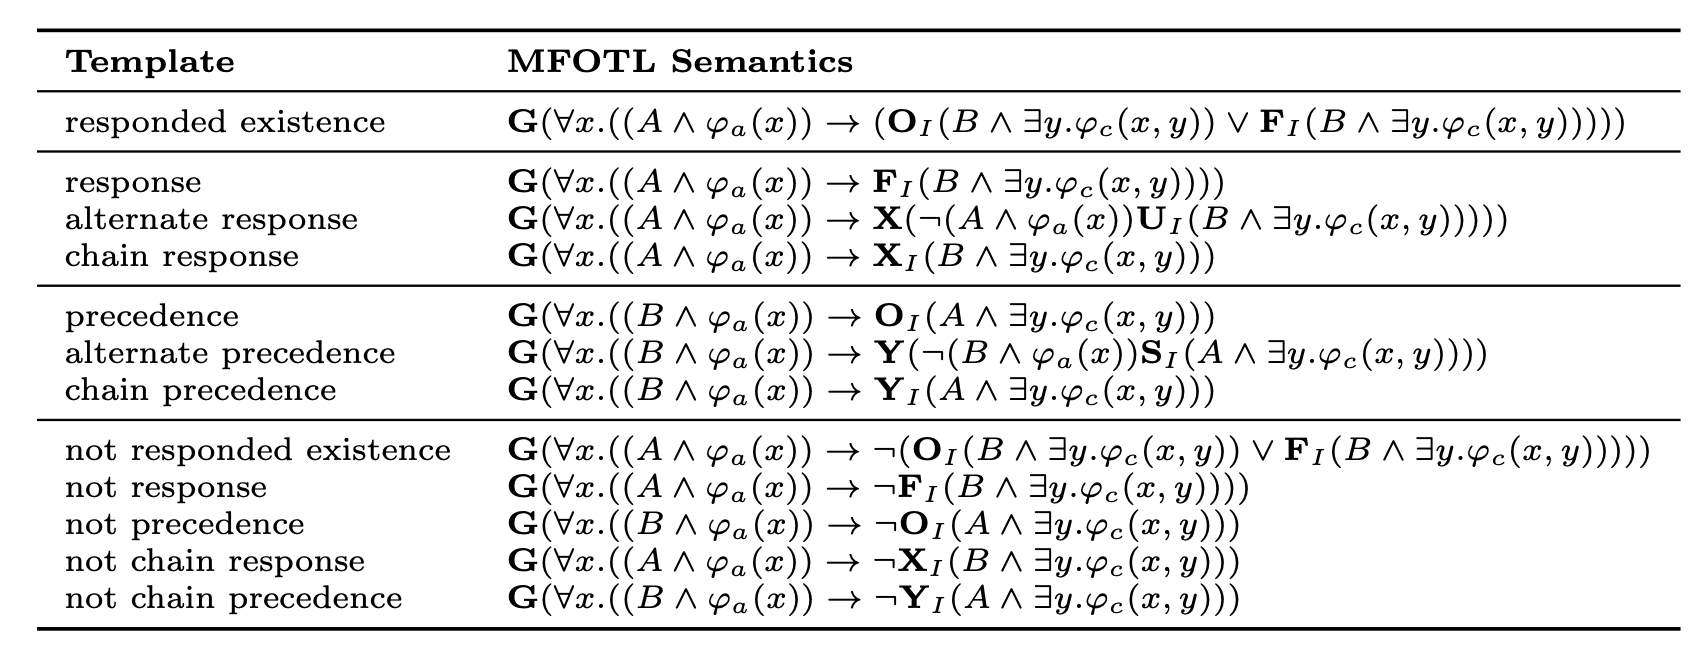
\includegraphics[scale=.3]{figures/mp-declare}
\end{center}



\end{frame}

%------------------------------------------------



\begin{frame}
\frametitle{Previous Work}

\begin{itemize}
	\item Monitoring solved for the propositional case~\cite{}
	\begin{itemize}
		\item Declare is a fragment of \ltl on finite traces (\ltlf)
		\item $\varphi$ has a corresponding FSA $\A_\varphi$ s.t. $\L(\A_\varphi)=\L(\varphi)$
		\item Technique based on \emph{coloring} $\A_\varphi$
		\item Essentially a  fixpoint computation on $\A_\varphi$
	\end{itemize}
\end{itemize}

\begin{itemize}
	\item Ultimate goal is lifting the technique to {\bf full MP-Declare}
	\item Currently focussing on {\bf data-only} fragment
\end{itemize}

\end{frame}

%------------------------------------------------

\begin{frame}
\frametitle{Solution for propositional case (\ltlf)}

Approach for propositional case (\ltlf)~\cite{}:  
\begin{enumerate}
	\item From $\varphi$, obtain $\A_\varphi$ (det, minimized)
	\item (Fixpoint computation)\\ 
		Assign one color to each $\A_\varphi$-state:
	\begin{itemize}
		\item \green{PS},\yellow{TS},\red{PV},\blue{TV}
	\end{itemize}
	\item Simulate $\A_\varphi$ on input $\tau$ and assign value according to current color
\end{enumerate}

~\\

Example:
\begin{itemize}
	\item $\varphi=\eventually p\lor \always(q\rightarrow\eventually r)$
	\item $\tau=\yellow{a}~\yellow{a}~\blue{q}~\blue{a}~\yellow{r}~\green{p}~\green{\cdots}$
\end{itemize}

\begin{center}
	%%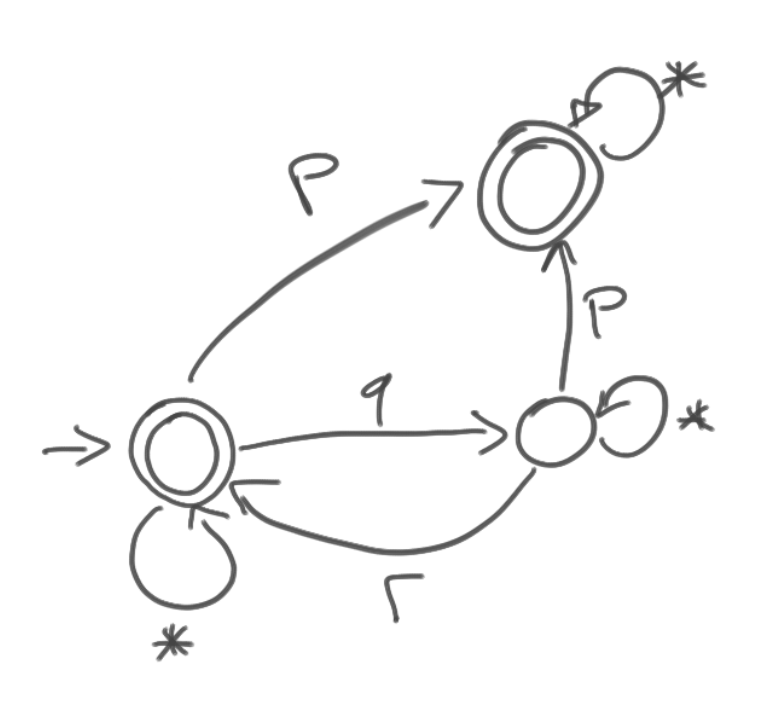
\includegraphics[scale=.2]{figures/a_phi}
	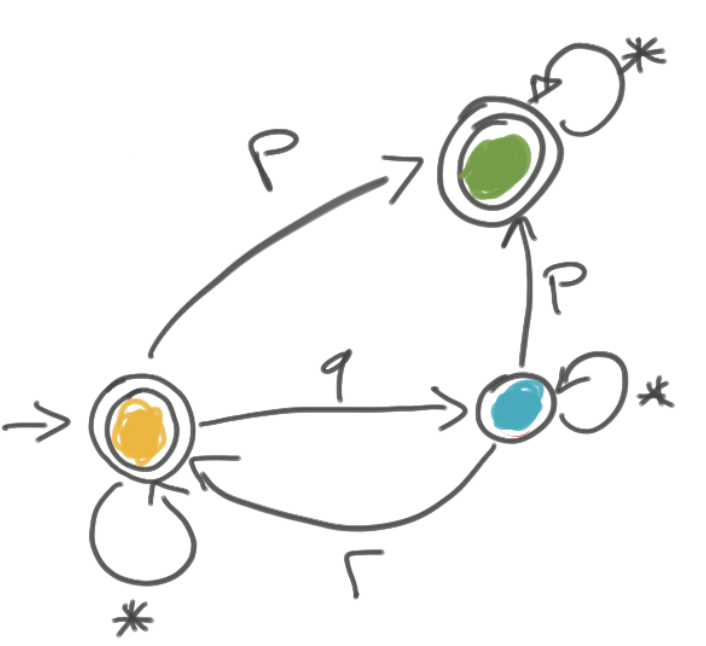
\includegraphics[scale=.2]{figures/a_phi_colored}
	%%
\includegraphics[scale=.2]{figures/color_codes}
\end{center}
\end{frame}

%------------------------------------------------

\begin{frame}
\frametitle{\ltlffo}

\ltlffo: lifting of \ltlf~to FO
\[
  \varphi ::=  \true \mid \phi  \mid \lnot \varphi \mid \varphi_1 \land \varphi_2 \mid \exists
  x.\varphi \mid \ltlX{\varphi}  \mid \varphi_1 \ltlU \varphi_2\text{ (}\phi:\text{ FO formula)} 
\]



\begin{itemize}	
	\item local properties are expressed in FOL
	\item across-state quantification allowed
	\item interpreted over finite traces of FO interpretations
\end{itemize}

\end{frame}

%------------------------------------------------
\begin{frame}
\frametitle{Data-only MP-Declare and \ltlffo}

\ltlffo captures data-only MP-Declare

\begin{center} 
	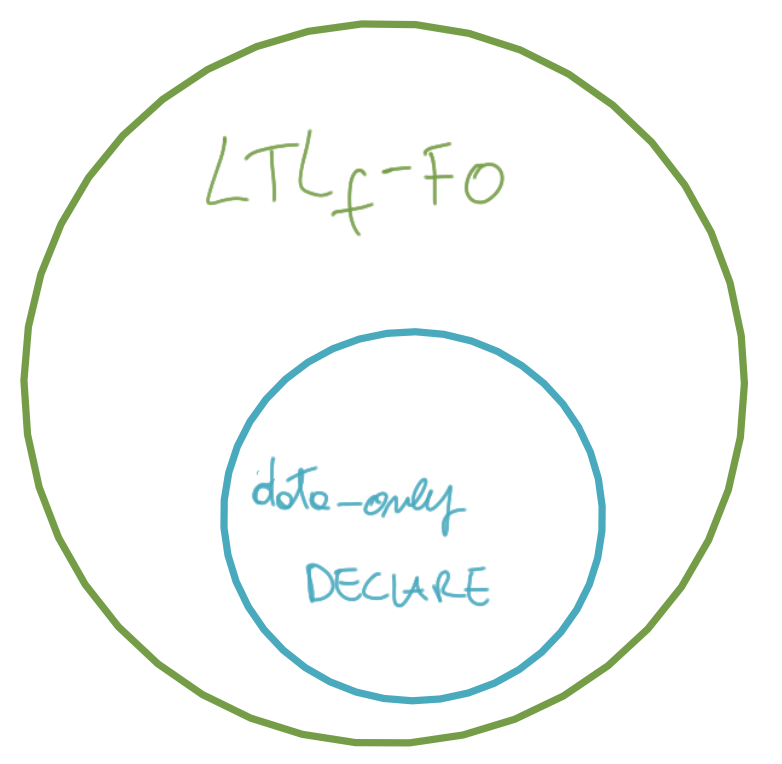
\includegraphics[scale=.15]{figures/ltl-declare}
\end{center}
%%
\begin{itemize}	
	\item Working with MP-Declare is difficult:
	\begin{itemize}	
		\item Templates, No recursive structure
		\item Must work ``by cases'', cannot use induction
	\end{itemize}
	
	\item \ltlffo is simpler, but:
	\begin{itemize}	
		\item more expressive
		\item undecidable~\cite{} both SAT and MC\\ 
			(does not imply MP-Declare undecidability)
	\end{itemize}
\end{itemize}


\end{frame}

%------------------------------------------------


\begin{frame}
\frametitle{\ltlffop}

We are focussing on the problem for 
\begin{center}
	\ltlffop: \emph{persistence-preserving} \ltlffo
\end{center}
%%
\[\varphi ::= \true \mid \phi \mid \lnot \varphi \mid \varphi_1 \land \varphi_2 \mid 
\exists \vec x.\live(\vec x)\land\varphi(\vec x) \mid
\live(\vec x)\land \ltlX\varphi(\vec x)  \mid\]
\[(\live(\vec x, \vec y)\land \varphi_1(\vec x)) \ltlU \varphi_2(\vec y)\]
%%
\begin{itemize}	
	\item $\live(x)$: object $x$ is in \emph{active domain}
	\item Quantification restricted only to objects that persist across states
\end{itemize}

The problem is now: Monitoring of  \ltlffop 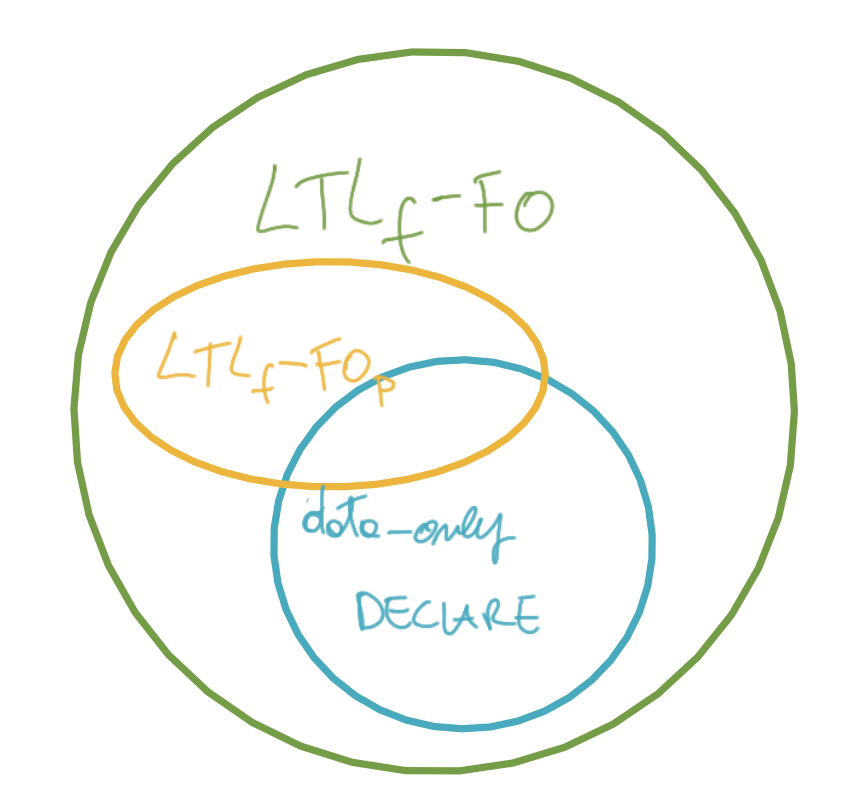
\includegraphics[scale=.2]{figures/ltlp-declare}

\end{frame}

%------------------------------------------------

\begin{frame}
\frametitle{From \ltlffop to \ltlf Monitoring}

We want to lift approach from \ltlf to \ltlffop

~\\

Obstacles: 
\begin{itemize}
	\item must define $\A_\varphi$ for the FO case
	\item $\A_\varphi$ must be effectively computable
\end{itemize}

~\\

Recall: 
\begin{itemize}
	\item activities carry a payload, i.e., $(A,1,2)$ instead of $A$
	\item payloads come from infinite domain (e.g., $\mathbb{N}$)
	\item $\A_\varphi$ must take payload into account ${}\rightarrow{}$ expect infiniteness
\end{itemize}
\end{frame}

%------------------------------------------------

\begin{frame}
\frametitle{From \ltlffop to \ltlf Monitoring}


\ltlffop  monitoring can be reduced to the propositional case

~\\


IDEA: 
\begin{itemize}
	\item satisfaction of \ltlffop formulae does not depend on \emph{actual objects}
	\item but on their \emph{mutual relationships}
\end{itemize}

~\\

Example ($\tilde{\cdot}$ stands for \emph{persistence-preserving} version):\\
$\varphi=\tilde\always(\forall x.((Pay\land\phi_a(x)) \rightarrow \tilde\eventually (Ship \land\exists y.\phi_c(x, y))))$,

\begin{itemize}
	\item $\phi_a\equiv item=x$ \text{ (\emph{activation} condition)}
	\item $\phi_c\equiv item= x \land address=y$ \text{(\emph{correlation} condition)}
\end{itemize}

\begin{itemize}
	\item $(\orange{Pay},10,\violet{shoes})~~~~(\sepia{DoSomething},\violet{shoes})~~~(\green{Ship},\violet{shoes},Park Avn)$
	\item $(\orange{Pay},1,\violet{gloves})~~~~(\sepia{DoSomething},\violet{gloves})~~(\green{Ship},\violet{gloves},Red Square)$
	\item $~~~(\orange{Pay},o_1,\violet{o_2})~~~~~~~~(\sepia{DoSomething},\violet{o_2})~~~~~~~~~~~~(\green{Ship},\violet{o_2},o_1)$
\end{itemize}
\end{frame}

%------------------------------------------------

\begin{frame}
\frametitle{From \ltlffop to \ltlf Monitoring}

\begin{definition}[p-equivalence]
Traces $\tau$ and $\tau'$ are \emph{p-equivalent} if obtained from each other through object renaming 
that preserves names of objects \ul{which persist between consecutive states}
\end{definition}

\begin{itemize}
	\item $(\orange{Pay},10,\violet{shoes})~~~~(\sepia{DoSomething},\violet{shoes})~~~(\green{Ship},\violet{shoes},Park Avn)$
	\item $~~~(\orange{Pay},o_1,\violet{o_2})~~~~~~~~(\sepia{DoSomething},\violet{o_2})~~~~~~~~~~~~(\green{Ship},\violet{o_2},o_1)$
	\item Crucial Observation: $o_1$ can be reused! (since not persisting)
\end{itemize}


\begin{theorem}
	\begin{enumerate}
		\item p-equivalent traces satisfy exactly same \ltlffop formulas
		\item $(2*max\_event\_arity)+1$ objects suffice to have a $\tau'$
			bisimilar to any $\tau$
	\end{enumerate}
\end{theorem}


\begin{itemize}
	\item we can work with \emph{equivalence classes} of events
	\item we can reduce to the case of \emph{finitely many} objects $\rightarrow$ propositional!
\end{itemize}
\end{frame}

%------------------------------------------------

\begin{frame}
\frametitle{From \ltlffop to \ltlf Monitoring}

Approach for \ltlffop: 
\begin{enumerate}
	\item Fix object domain $\hat\Delta=\{o_1,\ldots,o_{2m+1}\}$, 	for $m=max\_event\_arity$
	\item Compute $\hat\varphi$:\\ 
		~~~~propositional version of $\varphi$ (quantifier elimination with $\hat\Delta$) 
	\item Compute and color $\A_{\hat\varphi}$ (same as propostitional)
	\item\label{item:transform} Transform input $\hat\tau$ into p-bisimilar $\hat\tau$ over $\hat\Delta$, e.g.:
		\begin{itemize}
			\item $(\orange{Pay},10,\violet{shoes})~~~~(\sepia{DoSomething},\violet{shoes})~~~(\green{Ship},\violet{shoes},Park Avn)$
			\item $~~~(\orange{Pay},o_1,\violet{o_2})~~~~~~~~(\sepia{DoSomething},\violet{o_2})~~~~~~~~~~~~(\green{Ship},\violet{o_2},o_1)$
		\end{itemize}	
	\item\label{item:simulate} Simulate $\A_{\hat\varphi}$ on $\hat\tau$
\end{enumerate}

~\\

Steps \ref{item:transform} and \ref{item:simulate} can be applied incrementally:
\begin{itemize}
	\item process only last incoming event of $\tau$ (and $\hat\tau$)
	\item simulate only last transition in $\A_{\hat\varphi}$
\end{itemize}
\end{frame}

%------------------------------------------------

\begin{frame}
\frametitle{Complexity}

Complexity is triple-exponential:
\begin{enumerate}
	\item compute $\hat\varphi$: exponential wrt \# of quantified vars
	\item compute $\A_{\hat\varphi}$: doubly exponential wrt size of $\hat\varphi$ (exp in \# of q'ed vars)
	\item color $\A_{\hat\varphi}$: polynomial wrt size of $\A_{\hat\varphi}$ (doubly exp wrt size of $\hat\varphi$)
\end{enumerate}

~\\

Major obstacle, but:
\begin{itemize}
	\item $m$ typically small (arity is hardly large)
	\item in practice not much more difficult than propositional case
\end{itemize}

\end{frame}

%------------------------------------------------

\begin{frame}
\frametitle{Conclusions and Future Work}

Conclusions:
\begin{itemize}
	\item We are addressing monitoring of MP-Declare
	\item Currently focusing on data, \ltlffop
	\item Computability result based on abstraction technique
		\begin{itemize}
			\item inspired by related research line on FO $\mu$-calc~\cite{} (Model Checking)
		\end{itemize}
	\item Complexity is a major obstacle: 
		\begin{itemize}
			\item Need whole automaton to perform coloring
			\item but \# of objects typically small
		\end{itemize}
\end{itemize}

~\\

Future Work:
	\begin{itemize}
		\item Write the paper \smiley
		\item Assess practical impact of persistence-preservation wrt MP-Declare
		\item Implementation
		\item Evaluate additional complexity wrt propositional case in practice
	\end{itemize}


%% avoid minimization -> work with nfa -> can we adapt the coloring/monitoring algorihtm?
%% 


\end{frame}

%------------------------------------------------

\begin{frame}[allowframebreaks]
\frametitle{References}
\normalsize{
% \begin{thebibliography}{99} % Beamer does not support BibTeX so references must be inserted manually as below
% \bibitem[Smith, 2012]{p1} John Smith (2012)
% \newblock Title of the publication
% \newblock \emph{Journal Name} 12(3), 45 -- 678.
% \end{thebibliography}
\bibliographystyle{amsalpha}
\bibliography{biblio.bib}
}
\end{frame}

%----------------------------------------------------------------------------------------

\end{document} 

